\chapter{Experiments} % Results

This chapter presents simulation scenarios chosen to demonstrate the performance and limitations of the simulator, and to show the concept of OAL.

A common configuration for all experiments is given in table \ref{tab:var-allcases}. The individual configurations are presented in the respective sections.

\begin{table}
\centering
    \begin{tabular}{|c|c|c|}
        \hline
         \textbf{Description} & \textbf{Variable name} & \textbf{Value} \\
         \hline
         Link length $[m]$& \texttt{l} & $1$ \\
         \hline
         Link mass $[kg]$& \texttt{m} & $1$ \\
         \hline
         Obstacle safety radius $[m]$& \texttt{obstacle\char`_radius} & $0.1$\\
         \hline
    \end{tabular}
    \caption{Common simulation configuration for all cases}
    \label{tab:var-allcases}
\end{table}



%---------------------------------------------------------------------------------------
%---------------------------------------------------------------------------------------
%---------------------------------------------------------------------------------------

\section{Computed torque control}

This section briefly demonstrates how the robot behaves without the influence of obstacles in the environment.

\subsection{Case 1.1: Single reference}

Figure \ref{fig:case1-1} shows the different damping-cases of the computed torque controller following joint angle references. These references are plotted as dashed lines. The first and second case, with $\zeta = 0.3$ and $\zeta = 1$ respectively, are to demonstrate the potential of the controller. The last case, with $\zeta=2$, is the one used for the rest of the examples. A slow convergence is chosen to avoid abrupt movement, as there is no time criteria to be fulfilled. 

The damping ratio $\zeta=2$ together with $\mathbf{K_p} = 0.4 \mathbf{I}$ yields $\mathbf{K_d} = 2.5 \mathbf{I}$ following the relations in (\ref{eq:control2}).

\begin{figure}
    \centering
    
    \subfloat[Underdamped]{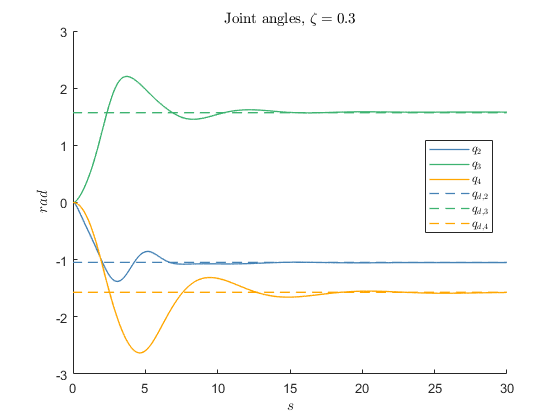
\includegraphics[totalheight=0.25\textheight]{figures/case-1-1/underdamped.png}}
    
    \subfloat[Critically damped]{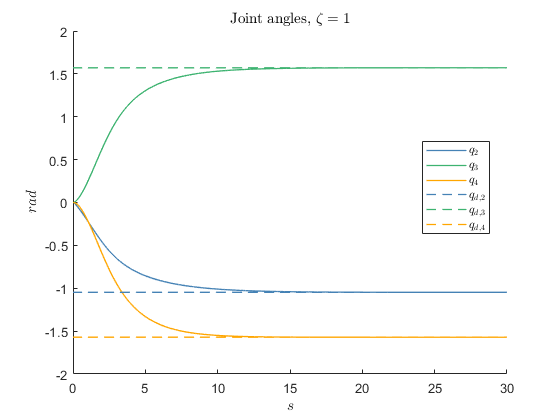
\includegraphics[clip=true, totalheight=0.25\textheight]{figures/case-1-1/criticallydamped.png}}

    \subfloat[Overdamped]{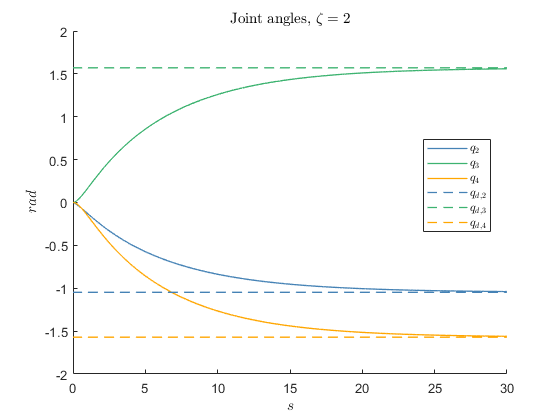
\includegraphics[clip=true, totalheight=0.25\textheight]{figures/case-1-1/overdamped.png}}

    \caption{Simulation demo - computed torque control}
    \label{fig:case1-1}
\end{figure}


%---------------------------------------------------------------------------------------
%---------------------------------------------------------------------------------------

\subsection{Case 1.2: Adjusting to path}

Plot joint angle ref med joint angle.
Vis sekvens.


%---------------------------------------------------------------------------------------
%---------------------------------------------------------------------------------------
%---------------------------------------------------------------------------------------

\section{OAL simulation scenarios}

\subsection{Case 2.1: Simple propulsion}

This scenario aims a demonstrating the concept of OAL. The snake robot is simply set to bend its front joint to $-\pi/2$. The other joints are to remain in a stretched out configuration. The simulator variable configuration can be seen in table \ref{tab:var-case-2-1}.
\begin{table}
\centering
    \begin{tabular}{|c|c|c|}
        \hline
         \textbf{Description} & \textbf{Variable name} & \textbf{Value} \\
         \hline
         Simulation time $[s]$& \texttt{simTime} & $20$ \\
         \hline
         Simulation sample time $[s]$& \texttt{h} & $0.001$ \\
         \hline
         Number of links & \texttt{n} & $4$ \\
         \hline
         Joint angle setpoints $[rad]$ & \texttt{q\char`_ref} & $[0, 0, 0, -\pi/2]$ \\
         \hline
         Initial joint angles $[rad]$ & \texttt{q\char`_0} & $[0, 0, 0, 0]$ \\
         \hline
         Number of obstacles & \texttt{num\char`_obstacles} & $3$ \\         
         \hline
         Obstacle positions $[m]$& \texttt{obstacle\char`_coords} & \makecell{$(0.8, -0.08)$ \\ $(1.6, 0.08)$ \\ $(3.3, -0.3)$} \\
         \hline
    \end{tabular}
    \caption{Simulation configuration for case 2.1}
    \label{tab:var-case-2-1}
\end{table}

The setpoints are manually set based on the knowledge that the bending link will collide with an obstacle in trying to fulfill the task. In order to obtain the desired angle, the link will apply a force to the obstacle underneath and consequently drag the whole robot body in the positive $x$ (rightward) direction. A sequence of the movement is presented in figure \ref{fig:case2-1}. The obstacles laying close to the rear links are positioned to allow the rest of the robot to stay flat. From the figure it can be seen that the robot moves away from the obstacles towards the end without pushing against any obstacles. This is a consequence of the modeled frictionless environment.

\begin{figure}
    \centering
    
    \subfloat[$t = 0 s$]{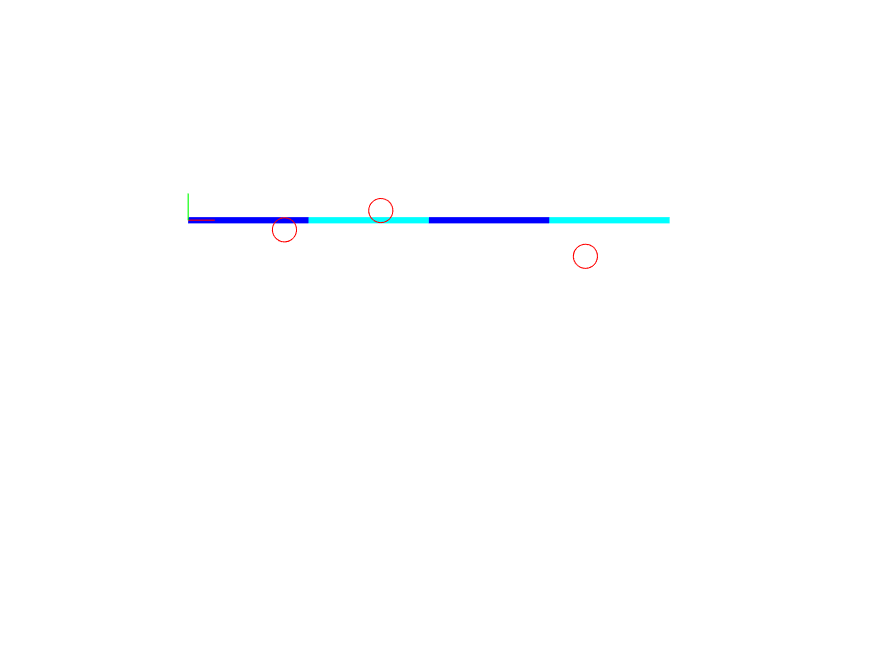
\includegraphics[trim=2cm 4cm 2cm 1.5cm, clip=true, totalheight=0.18\textheight] {figures/case-2-1/sim1.png}}
    \hfil
    \subfloat[$t = 4 s$]{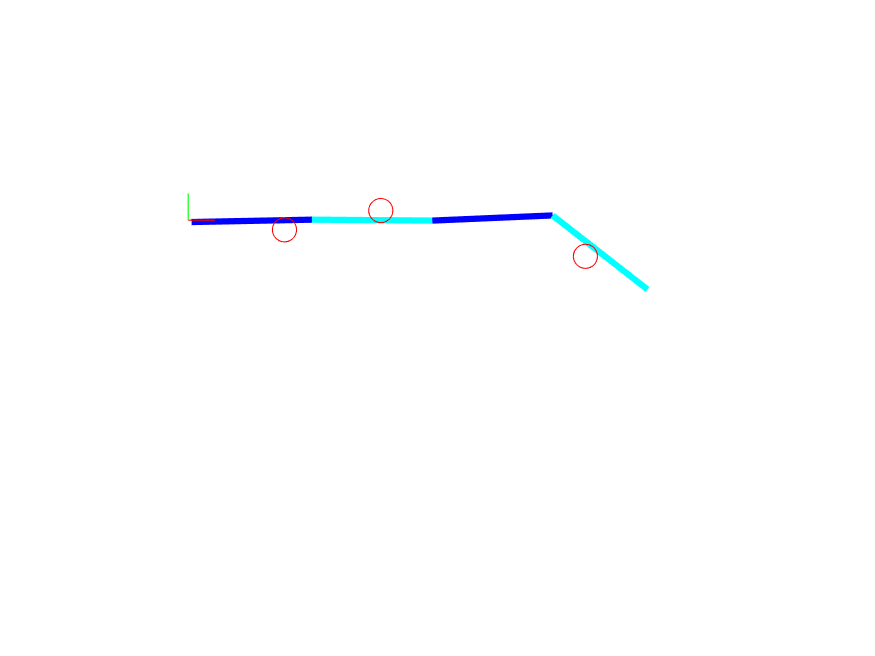
\includegraphics[trim=2cm 4cm 2cm 1.5cm, clip=true, totalheight=0.18\textheight]{figures/case-2-1/sim2.png}}
    
    \subfloat[$t = 8 s$]{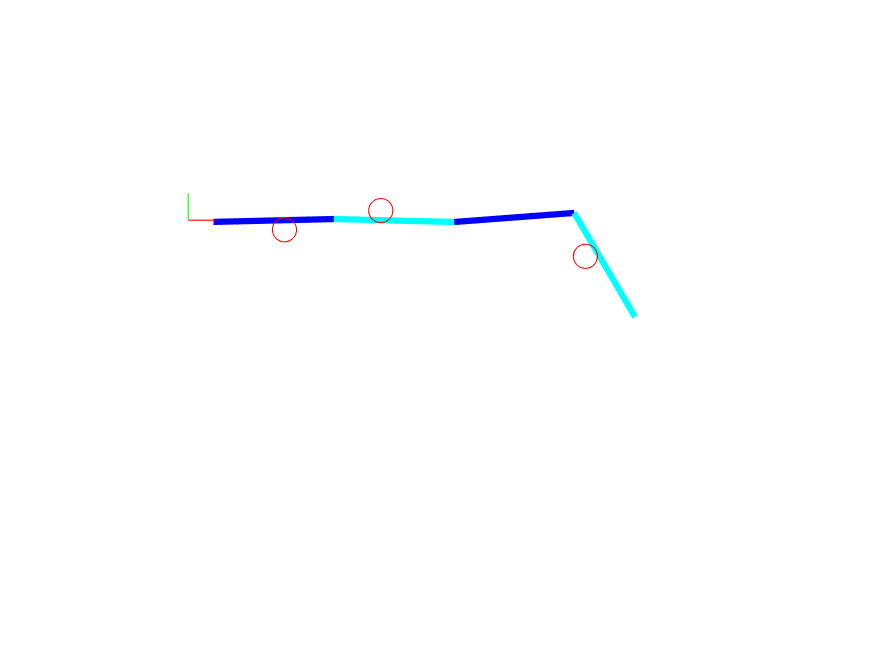
\includegraphics[trim=2cm 4cm 2cm 1.5cm, clip=true, totalheight=0.18\textheight]{figures/case-2-1/sim3.png}}
    \hfil
    \subfloat[$t = 12 s$]{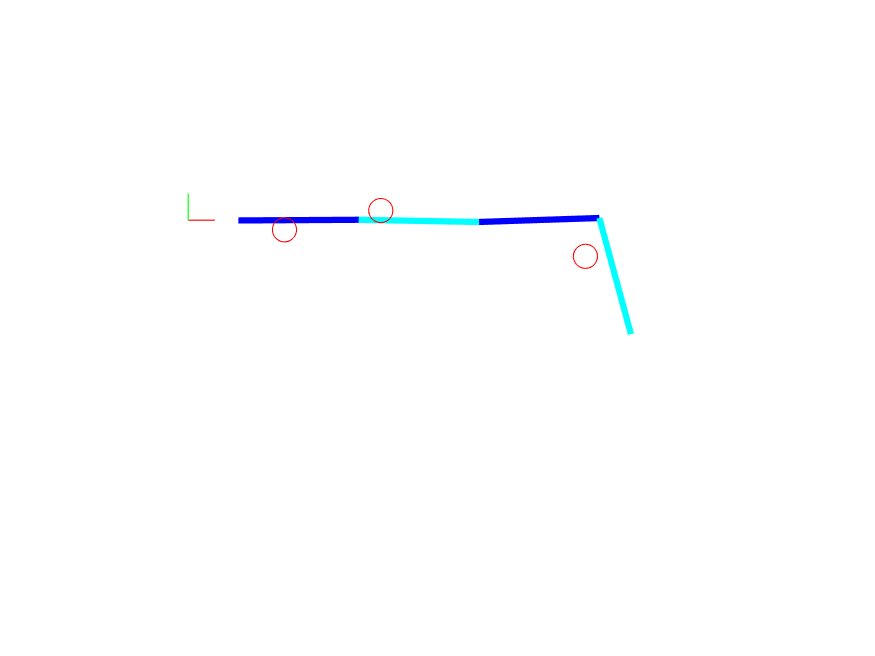
\includegraphics[trim=2cm 4cm 2cm 1.5cm, clip=true, totalheight=0.18\textheight]{figures/case-2-1/sim4.png}}

    \subfloat[$t = 16 s$]{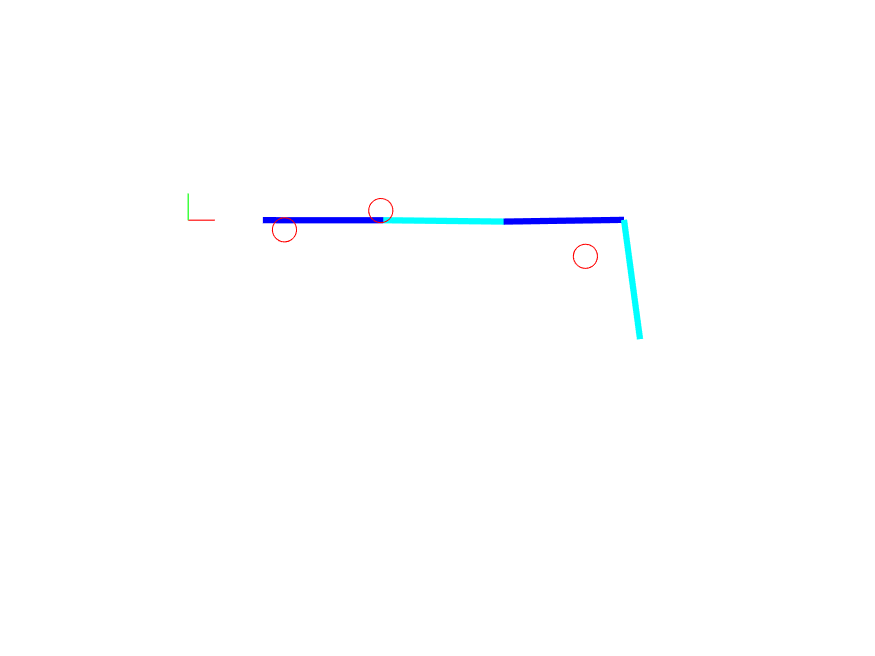
\includegraphics[trim=2cm 4cm 2cm 1.5cm, clip=true, totalheight=0.18\textheight]{figures/case-2-1/sim5.png}}
    \hfil
    \subfloat[$t = 20 s$]{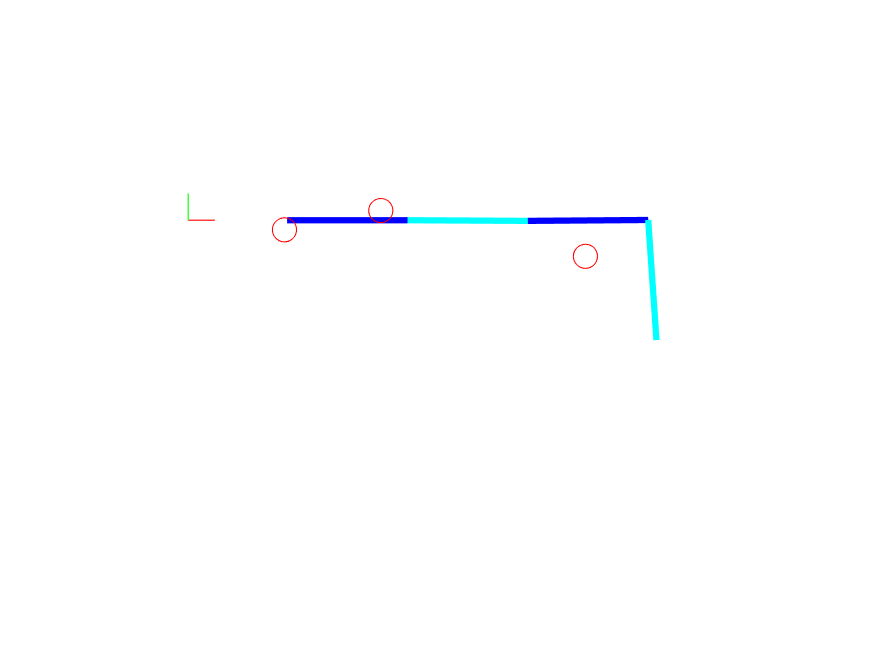
\includegraphics[trim=2cm 4cm 2cm 1.5cm, clip=true, totalheight=0.18\textheight]{figures/case-2-1/sim6.png}}

    \caption{Simulation demo - propulsion with static joint setpoint}
    \label{fig:case2-1}
\end{figure}

From the plots in figure \ref{fig:case2-1-plot} it is clear that the collision with the lower obstacle takes place at $~3 s$. At this point, the joint velocities are projected such that the link moves to the edge of the obstacle. Additionally, the preceding joints experience an offset as the last joint applies a torque that influences more than just the last link. This is evident in the frames (d) and (e) of figure \ref{fig:case2-1}.

\begin{figure}
    \centering
    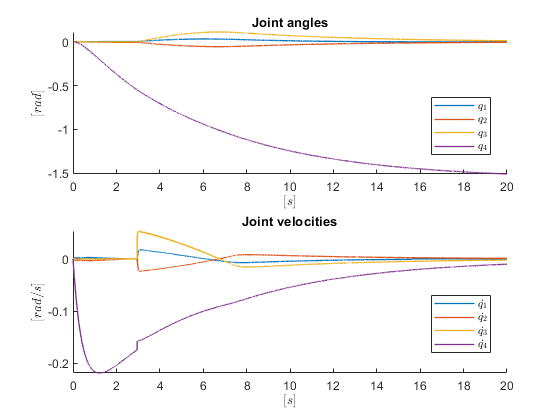
\includegraphics[width=0.9\textwidth]{figures/case-2-1/case2-1-joint-og-vel.png}
    \caption{Joint- angles and velocities for the single setpoint scenario}
    \label{fig:case2-1-plot}
\end{figure}

%---------------------------------------------------------------------------------------
%---------------------------------------------------------------------------------------

\subsection{Case 2.2: Propulsion infeasible}

As propulsion requires a force in the respective direction, there are scenarios where a set of obstacles are insufficient for attaining this force. This scenario aims at illustrating the case where the forces applied work against each other. The variable configuration for the simulation is presented in table \ref{tab:var-case-2-2}.

\begin{table}
\centering
    \begin{tabular}{|c|c|c|}
        \hline
         \textbf{Description} & \textbf{Variable name} & \textbf{Value} \\
         \hline
         Simulation time $[s]$& \texttt{simTime} & $9$ \\
         \hline
         Simulation sample time $[s]$ & \texttt{h} & $0.001$ \\
         \hline
         Number of links & \texttt{n} & $3$ \\
         \hline
         Joint angle setpoints $[rad]$& \texttt{q\char`_ref} & $[0, -\pi/3, \pi/3]$ \\
         \hline
         Initial joint angles $[rad]$& \texttt{q\char`_0} & $[0, 0, 0]$ \\
         \hline
         Number of obstacles & \texttt{num\char`_obstacles} & $3$ \\         
         \hline
         Obstacle positions $[m]$& \texttt{obstacle\char`_coords} & \makecell{$(0.5, 0.1)$ \\ $(1.5, -0.1)$ \\ $(2.5, 0.1)$} \\
         \hline
    \end{tabular}
    \caption{Simulation configuration for case 2.2}
    \label{tab:var-case-2-2}
\end{table}

Figure \ref{fig:case2-2} shows a sequence of the motion.

\begin{figure}
    \centering
    
    \subfloat[$t = 0 s$]{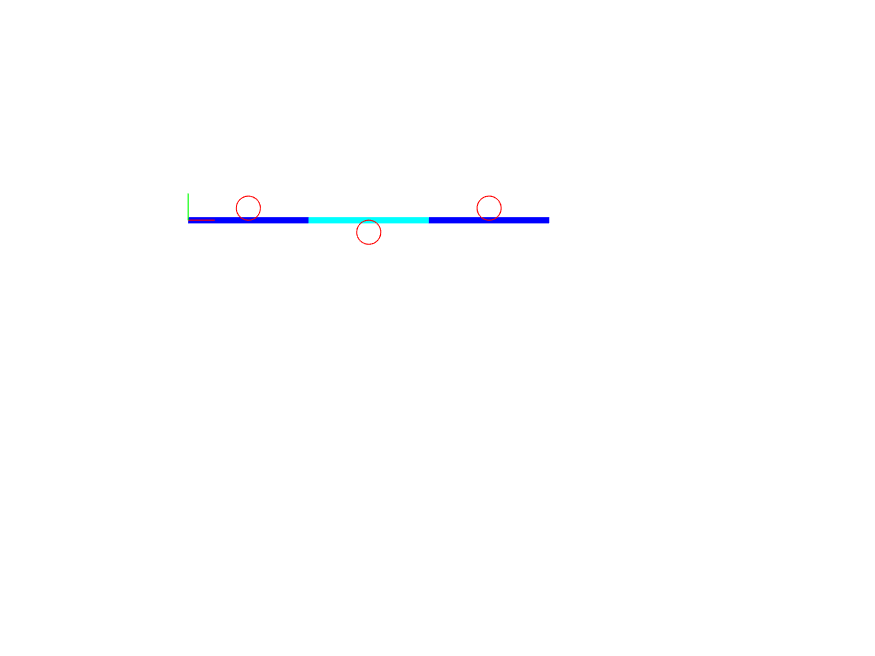
\includegraphics[trim=2cm 4cm 2cm 1.5cm, clip=true, totalheight=0.18\textheight] {figures/case-2-2/2sim1.png}}
    \hfil
    \subfloat[$t = 3 s$]{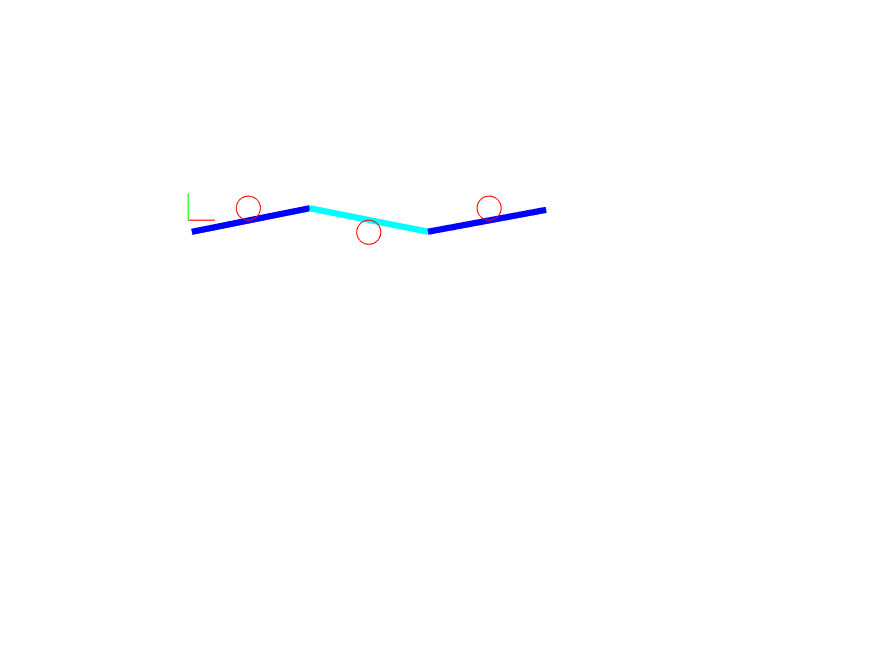
\includegraphics[trim=2cm 4cm 2cm 1.5cm, clip=true, totalheight=0.18\textheight]{figures/case-2-2/2sim2.png}}
    
    \subfloat[$t = 6 s$]{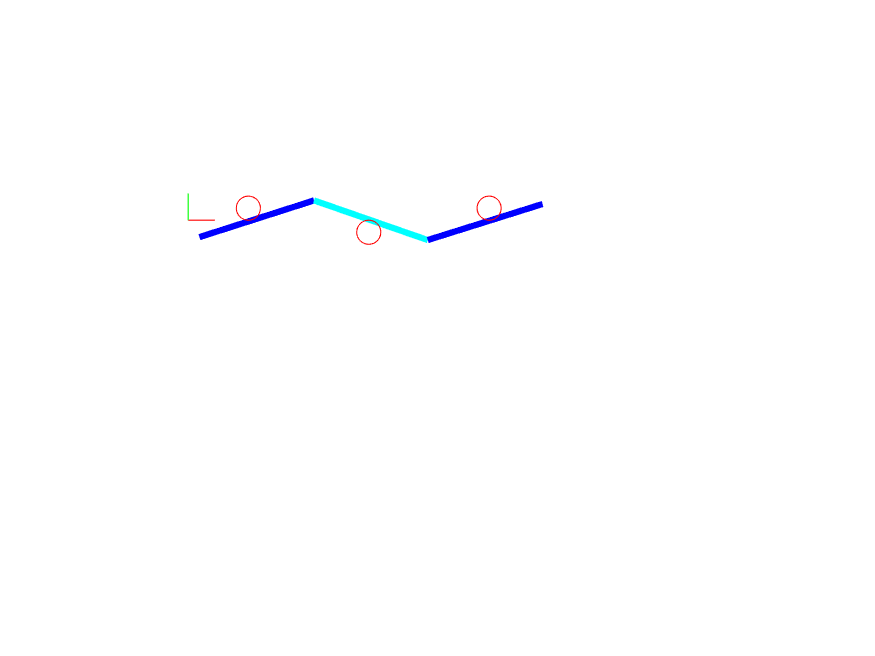
\includegraphics[trim=2cm 4cm 2cm 1.5cm, clip=true, totalheight=0.18\textheight]{figures/case-2-2/2sim3.png}}
    \hfil
    \subfloat[$t = 9 s$]{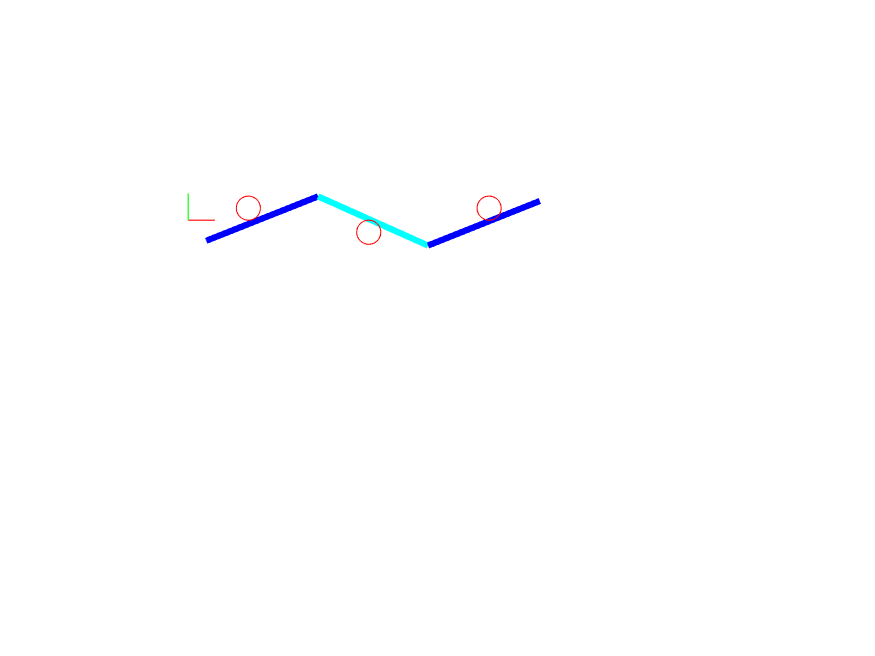
\includegraphics[trim=2cm 4cm 2cm 1.5cm, clip=true, totalheight=0.18\textheight]{figures/case-2-2/2sim4.png}}
    
    \caption{Simulation demo - no propulsion}
    \label{fig:case2-2}
\end{figure}

%---------------------------------------------------------------------------------------
%---------------------------------------------------------------------------------------

\subsection{Case 2.3: Propulsion along path}\label{subseq:case23}
Prøv med så magle lenker som mulig.
Vis sekvens. Plot av posisjon til hodet og path.

This case is to illustrate how the robot can aid obstacles to propel along a defined path. Since the robot is only position controlled based on deviation from the path, the obstacles are placed in a manner that supports both the desired shape and motion. This configuration can be seen in figure \ref{}. The two obstacles in the back are to keep the rear links on the path, while the obstacle in front is placed so that the robot can push against it and pull itself forward. In order for this to happen, the obstacle has been placed slightly on the path, leading to a constant error from the path. The robot's desire to always stay as close to the path as possible makes it push against the obstacle.

The variable configurations are presented in table \ref{tab:var-case-2-3}. The desired path is defined by (\ref{eq:path}), and consists of line segments and quadrants.

\begin{equation}\label{eq:path}
    y(x) =
    \begin{cases}
        0, & \text{if } x < 2.2 \\
        \sqrt{4 - (x - 2.2)^2}, & \text{if } x \in [2.2, 4.2] \\
        -\sqrt{4 - (x - 6.2)^2}, & \text{if } x \in [4.2, 6.2] \\
        -4, & \text{if } x > 6.2
    \end{cases}
\end{equation}
\\

\begin{table}
\centering
    \begin{tabular}{|c|c|c|}
        \hline
         \textbf{Description} & \textbf{Variable name} & \textbf{Value} \\
         \hline
         Simulation time $[s]$ & \texttt{simTime} & $240$ \\
         \hline
         Simulation sample time $[s]$ & \texttt{h} & $0.001$ \\
         \hline
         Number of links & \texttt{n} & $5$ \\
         \hline
         Joint angle setpoints $[rad]$& \texttt{q\char`_ref} & From path \\
         \hline
         Initial joint angles $[rad]$ & \texttt{q\char`_0} & $[0, 0, 0, 0, 0]$ \\
         \hline
         Number of obstacles & \texttt{num\char`_obstacles} & $3$ \\         
         \hline
         Obstacle positions $[m]$& \texttt{obstacle\char`_coords} & \makecell{$(0.8, -0.1)$ \\ $(1.6, 0.1)$ \\ $(3.2, -0.35)$} \\
         \hline
    \end{tabular}
    \caption{Simulation configuration for case 2.3}
    \label{tab:var-case-2-3}
\end{table}

The movement, as well as the desired path (red), is shown in figure \ref{}. It is clear that when the robot loses contact with the environment (at approximately 200 seconds), it has trouble with staying close to the path. Keep in mind that all movement is frictionless and that the robot therefore may keep on moving in a direction without simultaneously applying a force to the environment.

Robot moving slightly through obstacle radius towards the end.

\begin{figure}
    \centering
    
    \subfloat[$t = 0 s$]{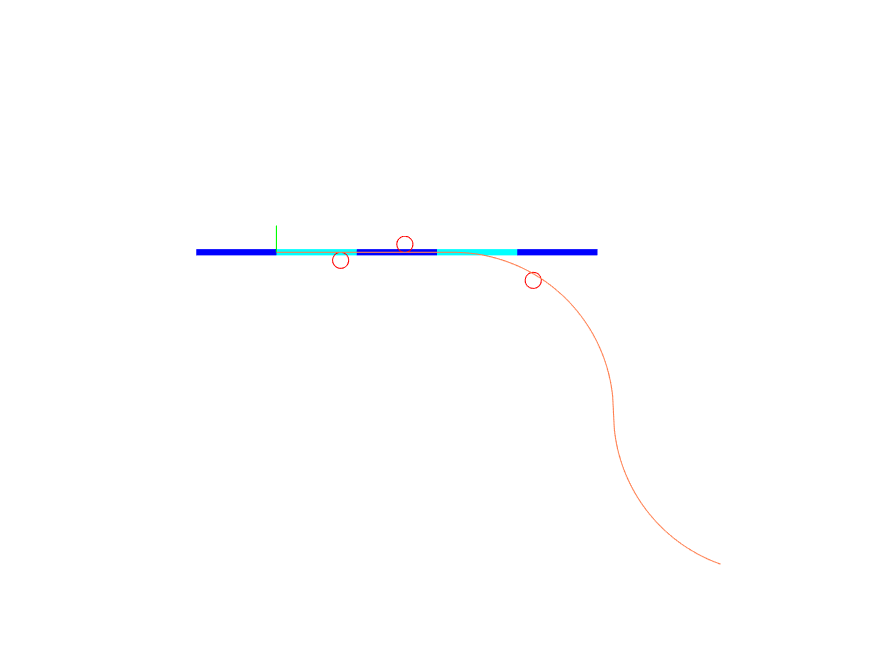
\includegraphics[trim=2cm 3cm 2cm 3cm, clip=true, totalheight=0.15\textheight] {figures/case-2-3/sim1.png}}
    \hfil
    \subfloat[$t = 40 s$]{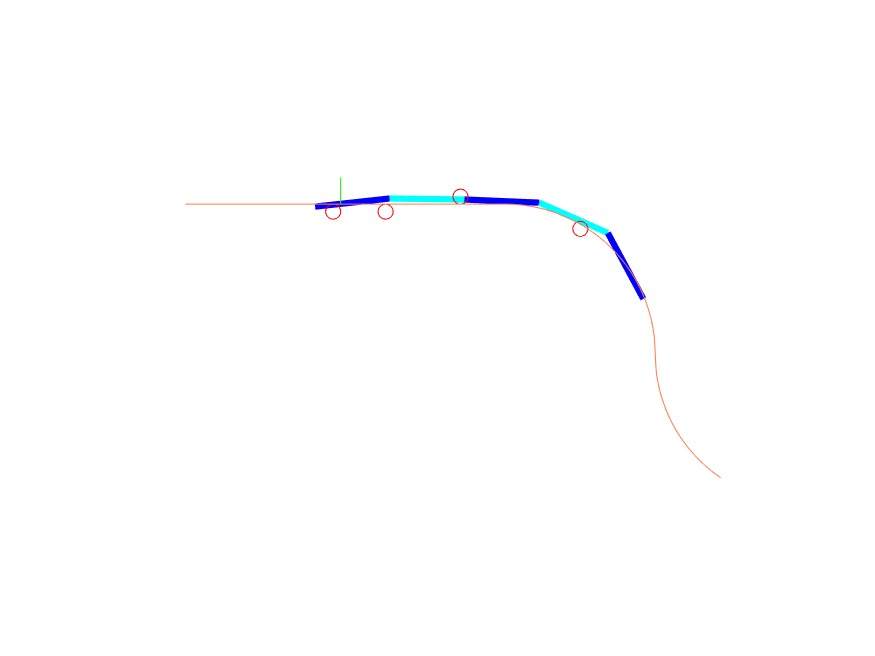
\includegraphics[trim=2cm 3cm 2cm 3cm, clip=true, totalheight=0.15\textheight]{figures/case-2-3/sim3.png}}
    
    \subfloat[$t = 80 s$]{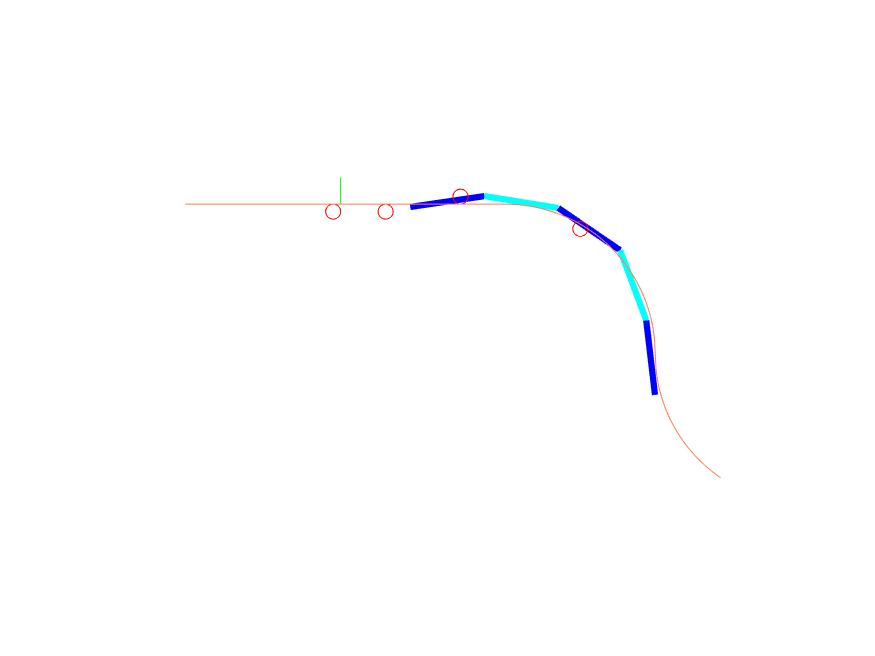
\includegraphics[trim=2cm 3cm 2cm 3cm, clip=true, totalheight=0.15\textheight]{figures/case-2-3/sim5.png}}
    \hfil
    \subfloat[$t = 120 s$]{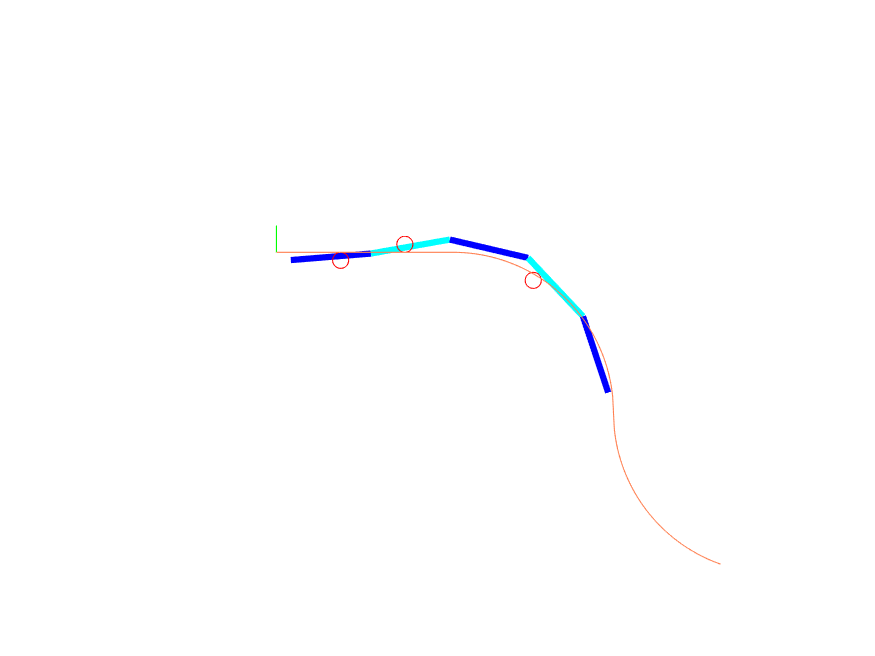
\includegraphics[trim=2cm 3cm 2cm 3cm, clip=true, totalheight=0.15\textheight]{figures/case-2-3/sim7.png}}

    \subfloat[$t = 160 s$]{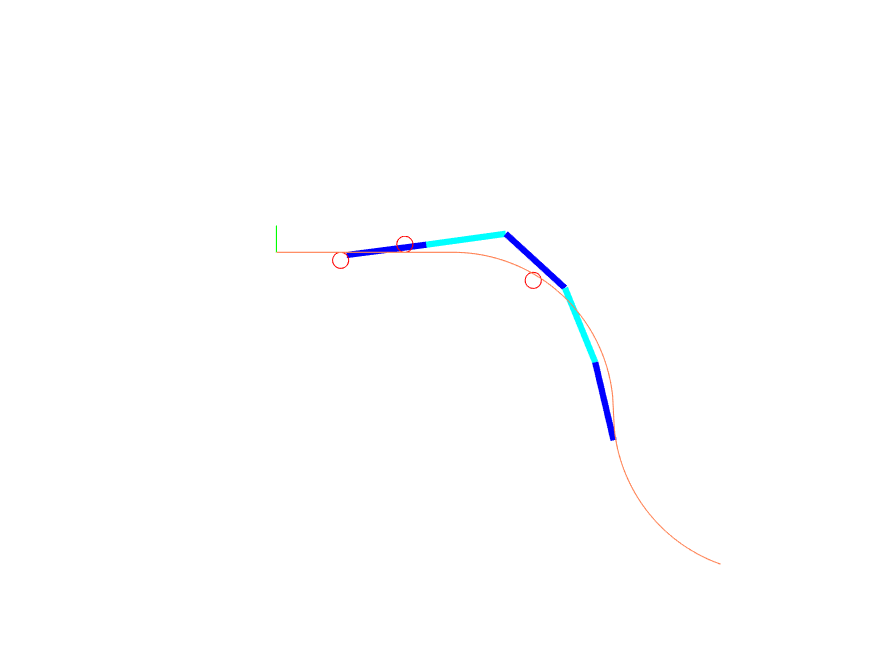
\includegraphics[trim=2cm 3cm 2cm 3cm, clip=true, totalheight=0.15\textheight]{figures/case-2-3/sim9.png}}
    \hfil
    \subfloat[$t = 200 s$]{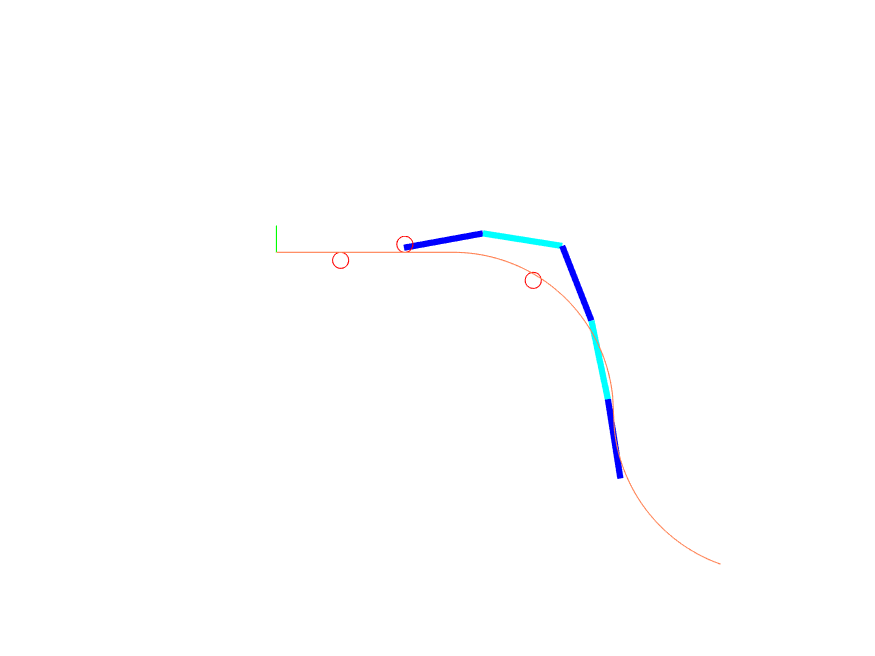
\includegraphics[trim=2cm 3cm 2cm 3cm, clip=true, totalheight=0.15\textheight]{figures/case-2-3/sim92.png}}
    
    \subfloat[$t = 220 s$]{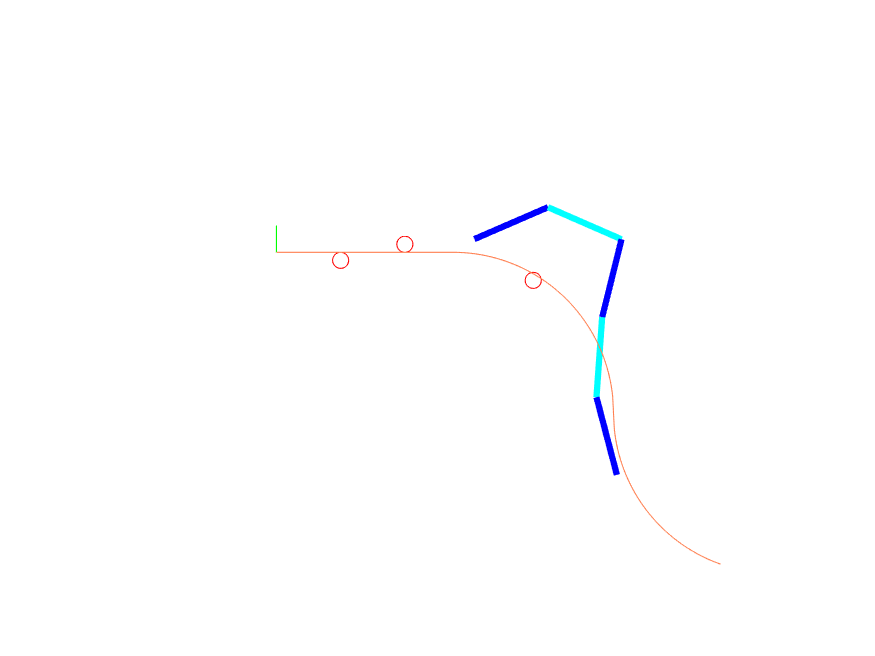
\includegraphics[trim=2cm 3cm 2cm 3cm, clip=true, totalheight=0.15\textheight]{figures/case-2-3/sim94.png}}
    \hfil

    \caption{Simulation demo - propulsion along path}
    \label{fig:case2-3}
\end{figure}

%---------------------------------------------------------------------------------------
%---------------------------------------------------------------------------------------

\subsection{Case 2.4: Unsuccessful propulsion attempt along path}
Robot går baklengst.
Vis sekvens. Plot av posisjon til hodet og path.

%---------------------------------------------------------------------------------------
%---------------------------------------------------------------------------------------
%---------------------------------------------------------------------------------------

